%\section{Phenomenological study of observables sensitive to the top
%quark mass}

\subsection{Definition of the observables}

We study the following observables:
\begin{itemize}

\item $m_{lb}$ -- which we define using the invariant mass squared
  \begin{equation}\label{def:mlb}
    \mlb^2\;=\;(p_l+p_b)^2
  \end{equation}
  where $p_l$ denotes the four-momentum of the lepton and $p_b$ the
  four-momentum of the $b$-jet. As there are two top quarks, there are also
 two possible \mlb\ values per event. Since experimentally, it is not possible to reconstruct
 the $b$-quark charge on an event-by-event basis with sufficient accuracy, one also needs a
 criterion to assign a pair of a charged lepton and a $b$-jet
 as the one stemming from the same top quark decay.
Following~\cite{Aaboud:2016igd}, the algorithm applied here is to choose
that $(l^+b\text{-jet},\,l^-b\text{-jet}')$ pairing which
 minimises the sum of the two \mlb\ values per event.
 Finally, the \mlb\ observable used in the analysis is the mean of the two \mlb\
 values per event obtained when applying the above procedure.

\item $m_{T2}$ -- which corresponds to the kinematic variable
  $m_{T2}$~\cite{Lester:1999tx,Barr:2003rg} that, applied to the
  $b\bar{b} 2l 2\nu$ final state, is defined as
  \begin{equation}\label{def:MT2}
    m_{T2}^2\;=\;\min_{\mathbf{p}_T^{\nu_1}+\mathbf{p}_T^{\nu_2}=\mathbf{p}_T^{\mrm{miss}}} \left[ \max \left\{ m_{T}^2 \left( \mathbf{p}_T^{(lb)_1}, \mathbf{p}_T^{\nu_1} \right), m_{T}^2 \left( \mathbf{p}_T^{(lb)_2}, \mathbf{p}_T^{\nu_2} \right) \right\}  \right].
  \end{equation}
Again the pairing of leptons and $b$-jets which minimises
$m_{(lb)_1}+m_{(lb)_2}$ is chosen.
The transverse mass is given by
\begin{equation}
m_T^2\left(\mathbf{p}_T^{(lb)_i}, \mathbf{p}_T^{\nu_i}\right) = m_{(lb)_i}^2 + 2 \left( E_T^{(lb)_i} E_T^{\nu_i} - \mathbf{p}_T^{(lb)_i} \mathbf{p}_T^{\nu_i} \right)\nonumber
\end{equation}
with $E_T = \sqrt{|\mathbf{p}_T|^2+m^2}$, where $m_{\nu_i} = 0$ was used.

\item $E_T^{\Delta R}$ -- which is defined as
  \begin{equation}\label{def:ETdR}
    E_T^{\Delta R}\;=\;\frac{1}{2}\,\left(E_T^{l_1}\Delta R(l_1,b_1)+E_T^{l_2}\Delta R(l_2,b_2)\right)
  \end{equation}
  using the above pairing criterion for leptons and $b$-jets.
  
\end{itemize}

We also consider the following fully leptonic observables, which are
part of the set of observables used for a recent top quark mass
determination from differential leptonic cross sections in Ref.~\cite{ATLAS-CONF-2017-044}:
\begin{itemize}

\item $m_{ll}$ -- as given by the invariant mass squared of the two charged
  leptons, defined as
  \begin{equation}\label{def:mll}
    \mll^2\;=\;(p_{l_1}+p_{l_2})^2~.
  \end{equation}
 
\item $p_{T,\mu}$ -- which is the transverse momentum of the muon.

\item $\eta_{\mu}$ -- which is the rapidity of the muon.

\end{itemize}


\subsection{Input parameters and event requirements}
\label{subsec:input}

We use the  PDF4LHC15\_nlo\_30\_pdfas
sets~\cite{Butterworth:2015oua,Dulat:2015mca,Harland-Lang:2014zoa,Ball:2014uwa}
and a centre-of-mass energy of $\sqrt{s}=13\tev$.
Our default top quark mass is  $m_t=172.5\gev$.
Leading order top quark and $W$ boson widths are used in the LO calculations and the NLO $t\bar{t}\, \otimes$ LO decay calculation, while NLO widths~\citep{Jezabek:1987nf} are used in the remaining NLO calculations.
Widths at NLO appearing in propagators are not expanded in \as{}.
The QCD coupling in the NLO widths is varied according to the chosen
scale. For \as{} evaluated at the central scale $m_t$, the numerical values for the widths are
\begin{equation}
\begin{matrix}
\Gamma_t^\mrm{LO} &=& 1.4806\gev{}&,&\quad \Gamma_t^\mrm{NLO} &=& 1.3535\gev{},\\
\Gamma_W^\mrm{LO} &=& 2.0454\gev{}&,&\quad \Gamma_W^\mrm{NLO} &=& 2.1155\gev{},\\
\Gamma_Z &=& 2.4952\gev{}&.& &&\\
\end{matrix}
\end{equation}
Jets are defined using the anti-$k_T$ algorithm~\cite{Cacciari:2008gp} as implemented in 
{\tt Fastjet}~\cite{Cacciari:2011ma}, with $R=0.4$.
For the electroweak parameters, we employ the following settings:
\begin{equation}\label{eq:ewparam}
  G_{\mu}\;=\;1.16637\cdot10^{-5}\gev{}^{-2},\quad
  M_{W} \;=\;80.385\gev{},\quad
  M_{Z} \;=\;91.1876\gev{}.
\end{equation}

Inspired by Ref.~\cite{Aaboud:2016igd}, and taking into account the
stronger trigger requirements for a $13\tev$ analysis, the following list
of event requirements is used. We require
\begin{itemize}
\item
  exactly two $b$-tagged jets with $p_T^\mrm{jet}>25\gev$ and
  $|\eta^\mrm{jet}|<2.5$. Jets containing a $b\bar{b}$ pair are also
  defined as $b$-jets.
\item
  exactly two oppositely charged leptons which fulfill
  $p_T^{\mu}>28\gev$, $|\eta^{\mu}|<2.5$ for muons and
  $p_T^{e}>28\gev$, $|\eta^{e}|<2.47$ for electrons excluding the
  range $1.37<|\eta^{e}|<1.52$.
  For both types of charged leptons with respect to any jet fulfilling
  the jet requirements, a separation of $\Delta R(l,\mrm{jet})>0.4$ is
  required.
\item
  $p_{T}^{lb}>120\gev$. Using the same lepton $b$-jet assignments as
  for $m_{lb}$, the observable $p_{T}^{lb}$ denotes the mean
  transverse momentum of the two lepton--$b$-quark systems.
\end{itemize}


The $b$-quarks are treated as massless in all fixed-order calculations.
We chose $\mu_R=\mu_F=m_{t}$ as our central scale. The impact of
choosing $H_T/2$ (rather than $m_t$) as the central scale on the top
quark mass determined by our method has been shown to be very
small~\cite{Heinrich:2013qaa}. It furthermore would be difficult to
facilitate an $H_T$ definition for the $\nlops$ approach that matches
the one used in the $\nlofull$ calculation. Even a simplified
$H_T$ definition that involved only the charged lepton and $b$-jet
transverse momenta and neglected the neutrino momenta would be
affected because the parton showering changes the $p_T$ spectrum of
the final state particles. We therefore considered it more consistent
to choose $m_t$ as the central renormalisation and factorisation scale
throughout all calculations. The scale variation bands are obtained by
varying $\mu_R$ and $\mu_F$ simultaneously by a factor of two and one
half with respect to the central scale.

For the parton shower results, we have also investigated the impact of
a dynamic scale, which we call $\mu_{t\bar t}$, 
to compute the matrix elements of the hard
scattering processes producing the top quark pairs.
The scale $\mu_{t\bar t}$ is a ``colour flow inspired'' QCD scale,  introduced
in Ref.~\cite{Hoeche:2013mua}. Using Mandelstam variables $s$, $t$ and
$u$, it is defined as
\begin{align}
  \mu_{t\bar t}^2(q\bar q\to t\bar t)&\;=\;2\,p_q p_t\;=\;m_t^2-t~,\nonumber\\[1mm]
  \mu_{t\bar t}^2(\bar qq\to t\bar t)&\;=\;2\,p_q p_t\;=\;m_t^2-u~,\nonumber\\[1mm]
  \mu_{t\bar t}^2(gg\to t\bar t)&\;=\;\left\{\begin{array}{ccl}
  m_t^2-t&&w_1\varpropto\,\frac{u-m_t^2}{t-m_t^2}+
    \frac{m_t^2}{m_t^2-t}\left\{\frac{4\,t}{t-m_t^2}+\frac{m_t^2}{s}\right\}\\
  &\text{with weight}&\\
  m_t^2-u&&w_2\varpropto\,\frac{t-m_t^2}{u-m_t^2}+
    \frac{m_t^2}{m_t^2-u}\,\left\{\frac{4\,u}{u-m_t^2}+\frac{m_t^2}{s}\right\}~.
  \end{array}\right.
  \label{eq:scale_ttb}
\end{align}
The value for the $gg$ partonic process is chosen randomly
according to the relative size of the two weights $w_1$ and $w_2$.

%--------------------------------------------------------------------------
\begin{table}[tb!]
\begin{center}
\begin{tabular}{|l|l|l|}
\hline&&\\[-3mm]
\multicolumn{1}{|c|}{\textbf{Scheme}} &
\multicolumn{1}{|c|}{\textbf{\boldmath Central scale $\mu_i$}} &
\multicolumn{1}{|c|}{\textbf{\boldmath Variations $\xi_i\,\mu_i$}}\\[1mm]
\hline&&\\[-5pt]
$\mu_F\mu_R\as{\mathrm{PS}}$ &
$\mu_F=\mu_R=\muqprod=\mt$, $\mu_R^\mrm{PS}=p_T^\mrm{emit}$ &
$\xi_R=\xi_F=\xi_R^\mrm{PS}=\{0.5,1.0,2.0\}$\\
&$\mu_F=\mu_R=\muqprod=\mu_{t\bar{t}}$, $\mu_R^\mrm{PS}=p_T^\mrm{emit}$&\\
&&\\[-6pt]
\hline&&\\[-5pt]
$\mu_F\mu_R\mu_Q$ &
$\mu_F=\mu_R=\muqprod=\mt$, $\mu_R^\mrm{PS}=p_T^\mrm{emit}$ &
$\xi_R=\xi_F=\{0.5,1.0,2.0\}$ and\\&&
$\hphantom{\xi_R=\,}\xi_Q=\{\sqrt2,1.0,1/\sqrt2\}$\\
&&\\[-6pt]
\hline&&\\[-5pt]
$\mu_F\mu_R\mu_Q\as{\mathrm{PS}}$ &
$\mu_F=\mu_R=\muqprod=\mt$, $\mu_R^\mrm{PS}=p_T^\mrm{emit}$ &
$\xi_R=\xi_F=\xi_R^\mrm{PS}=\{0.5,1.0,2.0\}$\\&&
and $\xi_Q=\{\sqrt2,1.0,1/\sqrt2\}$\\[-5pt]
&&\\
\hline
\end{tabular}
\end{center}
\caption{\label{tab:scalevars_nlops}%
  Summary of schemes employed to assess the scale variations in the
  $\nlops$ case. In all cases, the decay shower starting scale is kept
  constant, as given by its default $\muqdec=M_W/2$. Note that the
  local $p_T^\mrm{emit}$ values (squared) of each parton branching
  serve as the argument of $\as{}$ in the evaluation of the shower
  kernels. The related variation, $\xi_R^\mrm{PS}\,\mu_R^\mrm{PS}$,
  has been realised through appropriate adjustments of the
  \tsc{Sherpa} parameters {\tt CSS\_IS\_AS\_FAC} and {\tt CSS\_FS\_AS\_FAC}.}
\end{table}
%--------------------------------------------------------------------------

The standard $\mu_R$ and $\mu_F$ variations that we employ for our
fixed-order calculations are not fully appropriate to assess the
theory uncertainties of the $\nlops$ computations, as the
showering depends on further scale and parameter choices. For our
studies, it is interesting to vary $\muqprod$ as well as
$\muqdec$, which are the parameters controlling the overall size of
the resummation domains assigned to the $t\bar t$ production and top
quark decay showers, respectively. 
Within these resummation domains, subsequent shower emissions are
evaluated from the values taken by the ordering variable of the parton
shower.
We therefore also alter the strength
of the parton shower emissions by variations of 
$\mu_R^\mrm{PS}$, the scale entering the evaluation of the strong coupling
$\as{}(\mu_R^\mrm{PS})$ used in the shower kernels. For the
\tsc{Sherpa}~\tsc{CSshower}, the ordering variable is associated with
the local $p_T^\mrm{emit}$ scales of the individual branchings, which
means $\mu_{R,k}^\mrm{PS}\sim p_{T,k}^\mrm{emit}$ for the $k$-th branching.
%
For the combined variation of several
$\nlops$ parameters, we follow the principle of identifying the
strongest and weakest shower option that one can possibly obtain from
the given individual parameter ranges. This is supposed to lead to a
conservative shower uncertainty estimate.

Our default variation in the $\nlops$ case, denoted by
$\mu_F\mu_R\as{\mathrm{PS}}$, is a
combination of simultaneously varying $\mu_F, \mu_R$ and $\mu_R^\mrm{PS}$ by a factor of
two up and down, with central scale $\mt$.
Alternative ways of uncertainty assessment include the variation of $\muqprod$ and $\muqdec$. 
The \tsc{Sherpa} default is to set  $\muqprod$  equal to
the factorisation scale, while the starting scale of the decay shower
is set to $\muqdec=M_W/2$ and not varied.\footnote{%
  The top quark decays induce a deflection of the colour flow of the
   top quark. The scale of the deflection on average
  corresponds to the mass of the $W$ boson, which therefore serves as
  an appropriate choice for the scale associated with the
  first decay shower branching.}
The different scale variation schemes, which are used by us in the $\nlops$ case are summarised in Table~\ref{tab:scalevars_nlops}.
For each of the schemes shown in Table~\ref{tab:scalevars_nlops}, the uncertainty bands are defined as
the maximum deviation from the central prediction on either side.


\subsection{Numerical predictions}

\subsubsection{Comparison of the different theoretical descriptions}

\begin{table}
\centering
\begingroup
\def\arraystretch{1.3}
\begin{tabular}{|c|c|c|}
\hline
& X=LO $\left[\mathrm{fb}\right]$ & X=NLO $\left[\mathrm{fb}\right]$\\
\hline
$\mathbf{X_{full}}$ & $\left( 739.5\pm   0.3\right)^{ + 31.5\%}_{-22.4\%}$ & $\left( 914\pm   3\right)^{ +  2.1\%}_{ -7.6\%}$\\
$\mathbf{X_{NWA}^{LOdec}}$& $\left( 727.3\pm   0.2\right)^{ + 31.4\%}_{-22.3\%}$ & $\left( 1029\pm   1\right)^{ + 10.4\%}_{-11.5\%}$\\
$\mathbf{X_{NWA}^{NLOdec}}$ & - & $\left( 905\pm   1\right)^{ +  2.3\%}_{ -7.7\%}$\\
$\mathbf{X_{PS}}, \mu=m_t$ & $\left( 637.7\pm   0.9\right)^{ + 29.7\%}_{-21.0\%}$ & $\left( 886\pm   1\right)^{ +  8.5\%}_{ -9.3\%}$\\
$\mathbf{X_{PS}}, \mu=\mu_{t\bar{t}}$ & $\left( 499.7\pm   0.7\right)^{ + 27.6\%}_{-19.3\%}$ & $\left( 805.2\pm   0.9\right)^{ + 12.3\%}_{-10.9\%}$\\
\hline
\end{tabular}
\endgroup
\caption{\label{tab:xs}%
  Fiducial cross sections in various approximations. The first
  uncertainty is the precision of the Monte Carlo phase space integration.
  The scale variation uncertainty obtained by simultaneously varying
  renormalisation and factorisation scales by a factor of two
  (superscript) and one half (subscript) is given in percent.
  For the parton shower results, the  given scale uncertainties are
  obtained by using the variation prescription $\mu_F\mu_R\as{\mathrm{PS}}$
  as detailed in the text.}
\end{table}

In this section, we compare four different NLO descriptions of the $(e^+ \nu_e)\,(\mu^- \bar{\nu}_{\mu})\,b\bar b$ final state
for the  observables described in Section~\ref{sec:calculation}.
Some of the purely leptonic observables have also been used by the ATLAS collaboration
for their recent top quark mass determinations based on $8\tev$ data presented in Ref.~\cite{ATLAS-CONF-2017-044}.
Aiming to quantify the relative differences of the theoretical descriptions,
which should only mildly depend on the centre-of-mass energy,
we show results at the present LHC setting of $13\tev$.
The corresponding fiducial cross sections are summarised in Table~\ref{tab:xs}.
While the level of agreement between the fixed-order full and NWA
calculations is as expected, considerably smaller cross
sections are obtained for the parton shower calculations. Showering leads to a softening
of the final state $b$-jets. In turn, a good fraction of them no longer
satisfy the jet requirements, resulting in an event loss.
The parton shower computation
with $\mu=\mu_{t\bar t}$ leads to an even stronger amount of
radiation, and consequently to a further loss of events due to
insufficiently energetic $b$-jets.

\begin{figure}[tbp!]
\centering
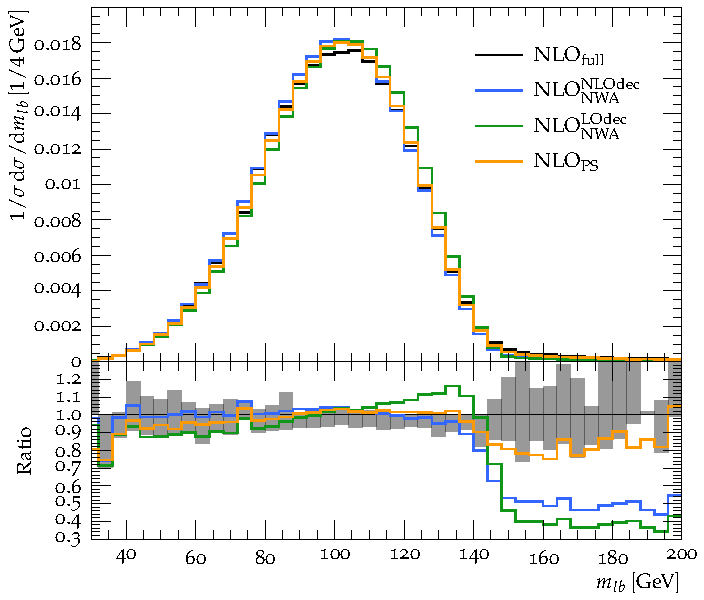
\includegraphics[width=0.8\textwidth]{{plots/scalevarcompare.mlb}.pdf}
\caption{\label{fig:scalevar_mlb}%
  Normalised differential cross sections for the invariant mass
  $m_{lb}$ at the $13\tev$ LHC for four different theoretical
  descriptions: $\nlofull$, $\nlodec$, $\lodec$ and $\nlops$. The ratios
  of all descriptions to $\nlofull$ including its scale uncertainty
  band are also shown.}
\end{figure}

In Fig.~\ref{fig:scalevar_mlb}, we present the normalised differential cross sections for $m_{lb}$ based on the four theoretical descriptions,
evaluated at  $\mu_R=\mu_F=m_t$.
In the lower part of the figure, we show their ratio to the $\nlofull$ prediction, including an uncertainty band from
scale variations by a factor of two and one half with respect to the central scale.
We find that 99\% of the total fiducial cross section is accumulated in the range $40$--$150\gev$.
A kinematic edge at $m_{lb}^\mrm{edge}=\sqrt{m_t^2-M_W^2}=152.6\gev$ leads to a sharp drop in the distribution
beyond which it is only populated by non-resonant contributions, additionally clustered radiation and incorrect $b$-lepton pairings.
The significantly larger scale uncertainty for $m_{lb}\ge150\gev$ is due to the fact that NLO is the first non-trivial order populating this region.
This conclusion is further substantiated by the sizeable perturbative correction that we discuss in the following section.
Hence, resummation effects are expected to play a larger role in the vicinity of this kinematic boundary.

We now discuss the impact of off-shell and non-resonant contributions on the $m_{lb}$ distribution.
Their effect is easiest seen by discussing $\nlodec$, displayed in the lower part of Fig.~\ref{fig:scalevar_mlb}.
In the range $30\gev\le\mlb\le130\gev$ the description of this prediction agrees with the full calculation to within a few percent.
The deviations are barely visible within the statistical fluctuations. Around the peak region of the differential cross section for $m_{lb}$, the
NWA calculation overshoots by about 4\%.
This level of agreement is to be expected given the parametric suppression of off-shell effects by $\Gamma_t \big/ m_t$,
which is mildly violated by the applied phase space restrictions.
For $m_{lb}\ge130\gev$, the difference between $\nlodec$ and $\nlofull$ starts to grow
and saturates at about $-50$\% for $\mlb$ values larger than $m_{lb}^\mrm{edge}$.
Again, this is to be expected as the NWA does not apply in this part of the phase space.
In fact, the $\lolo$ prediction (not shown in Fig.~\ref{fig:scalevar_mlb}) vanishes for $m_{lb}\ge m_{lb}^\mrm{edge}$.


\begin{figure}[tbp!]
\centering
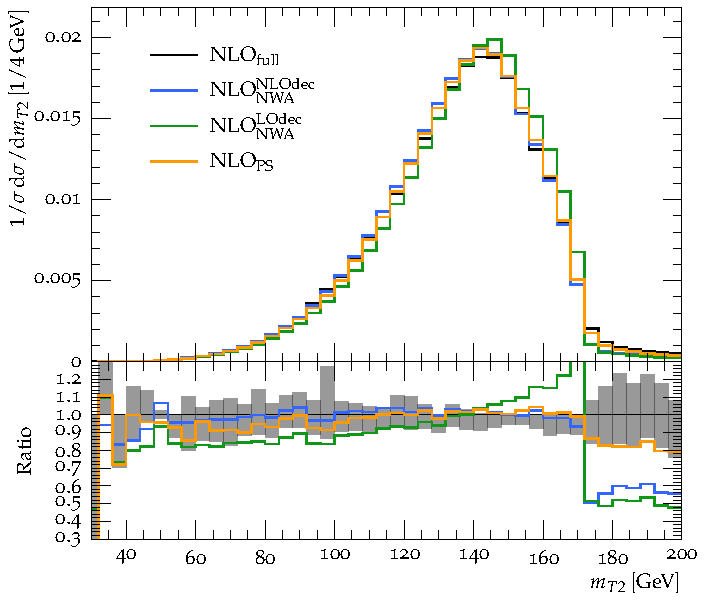
\includegraphics[width=0.8\textwidth]{{plots/scalevarcompare.mt2}.pdf}
\caption{\label{fig:scalevar_all_mt2}%
  Normalised differential cross sections for the $m_{T2}$ observable
  at the $13\tev$ LHC, analogous to Fig.~\ref{fig:scalevar_mlb}.
  The ratios of different theoretical descriptions to $\nlofull$
  including its scale uncertainty band are also shown.}
\end{figure}

It is also interesting to study the $\lodec$ prediction to investigate the importance of NLO corrections to the top quark decay.
We find  significant shape differences compared to the full
calculation of the order of about $-10$\% for $\mlb$ around
$50\gev$, rising to about $+20$\% around $\mlb\sim140\gev$.
For $m_{lb}\ge m_{lb}^\mrm{edge}$, the description completely fails.
Therefore, it is crucial in the application of the NWA to account for a fully consistent NLO treatment of production {\em and} decay.
Comparing $\nlops$ with $\lodec$, we find that the parton shower treatment of the top quark decay
drives the shape more towards the $\nlofull$ case for $\mlb>m_{lb}^\mrm{edge}$.
For low \mlb values, the parton shower result mostly lies
between the $\lodec$ and $\nlodec$ predictions.

Finally, we discuss the shape differences introduced by the different descriptions in the light of the scale uncertainties.
For clarity of the presentation, we only show the scale band of the
$\nlofull$ reference prediction in the lower part of
Fig.~\ref{fig:scalevar_mlb}.
For the other cases, we refer to Section~\ref{subsec:scaledep}.
We observe that in the bulk of the distribution, shape differences of $\nlodec$ with respect to $\nlofull$ lie inside
the uncertainty bands.
In contrast, both $\lodec$ and $\nlops$ exhibit differences to $\nlofull$ outside their respective
uncertainty bands, $\nlops$ however being much closer to $\nlofull$
than $\lodec$  (see also Fig.~\ref{fig:mlb_scalevar_nwa}).

\begin{figure}[tbp!]
  \centering
  \begin{subfigure}{0.495\textwidth}
    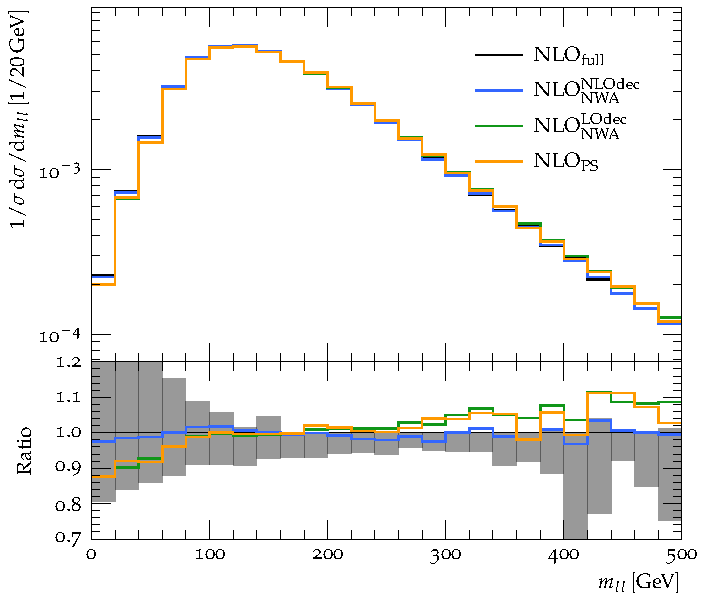
\includegraphics[width=\textwidth]{{plots/scalevarcompare.mll}.pdf}
    \vspace{\TwoFigBottom em}
    \caption{\label{fig:scalevar_all_mll}}
  \end{subfigure}
  \hfill
  \begin{subfigure}{0.495\textwidth}
    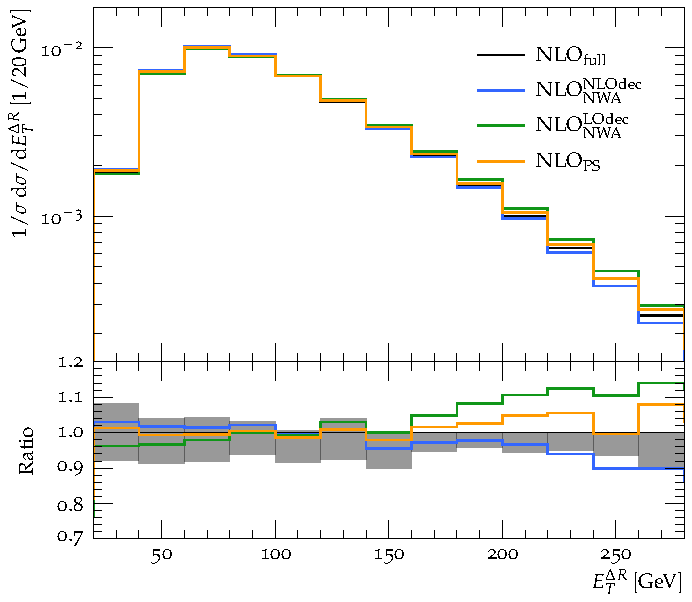
\includegraphics[width=\textwidth]{{plots/scalevarcompare.etdr}.pdf}
    \vspace{\TwoFigBottom em}
    \caption{\label{fig:scalevar_all_etdr}}
  \end{subfigure}
  \caption{Normalised differential cross sections for (a)~the
    di-lepton invariant mass, \mll, and (b)~the observable \etdr.
    The ratios of the different theoretical descriptions to $\nlofull$
    including its scale uncertainty band are also shown.}
\end{figure}

In Fig.~\ref{fig:scalevar_all_mt2}, we show the normalised distribution of $m_{T2}$ as defined in Eq.~(\ref{def:MT2}), for the four theoretical descriptions.
By construction, this observable has a sharp kinematic edge at $m_{T2}=m_t$, which is clearly visible and mildly washed out
by off-shell effects, ambiguities related to missing energy and jet recombination.
We find that for the $\nlofull$ prediction, 97\% of the total fiducial cross section is contained below $m_{T2}\le m_t$.
The shapes of the different theoretical descriptions follow patterns very similar to those observed for $m_{lb}$.
In particular, the $\nlodec$ prediction closely follows $\nlofull$ up to the kinematic edge,
with shape differences of a few percent, but in general within the scale uncertainty band.

In Fig.~\ref{fig:scalevar_all_mll}, we show the di-lepton invariant mass $m_{ll}$.
We observe that off-shell effects are small and that all theoretical
descriptions agree at the 10\% level.
This is expected because $\mll$ is an observable which is inclusive in what concerns extra radiation.
The descriptions $\lodec$ and $\nlops$ show a very similar behaviour
and are outside the uncertainty bands of the $\nlofull$ prediction
except for low $\mll$ values.
In Fig.~\ref{fig:scalevar_all_etdr}, we display the \etdr observable defined in Eq.~(\ref{def:ETdR}).
Similar to \mll, also for \etdr, the $\nlofull$ and $\nlodec$
predictions do not exhibit large differences.
However, the shapes of the $\lodec$ and $\nlops$ predictions differ considerably from the  $\nlofull$ prediction.
In contrast to the \mll case, the $\lodec$ and $\nlops$ predictions also differ significantly from each other.

\begin{figure}[tbp!]
\centering
\begin{subfigure}{0.495\textwidth}
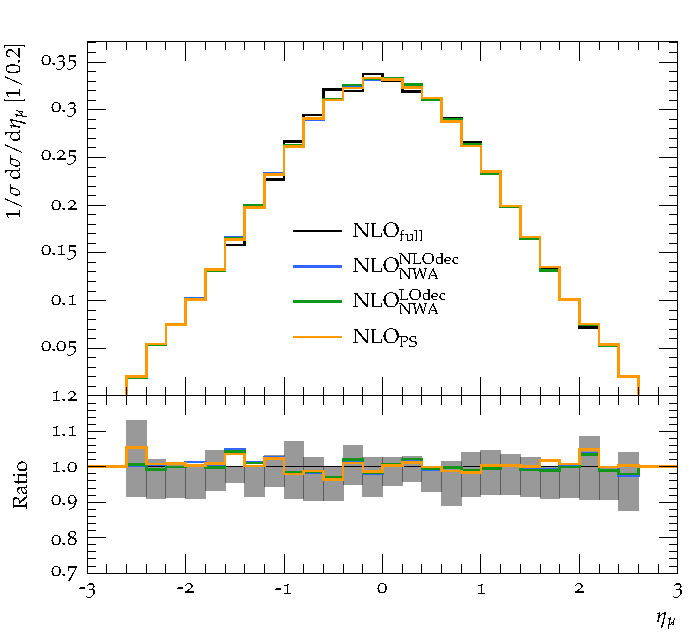
\includegraphics[width=\textwidth]{{plots/scalevarcompare.etamu}.pdf}
\vspace{\TwoFigBottom em}
\caption{\label{fig:scalevar_etamu}}
\end{subfigure}
\hfill
\begin{subfigure}{0.495\textwidth}
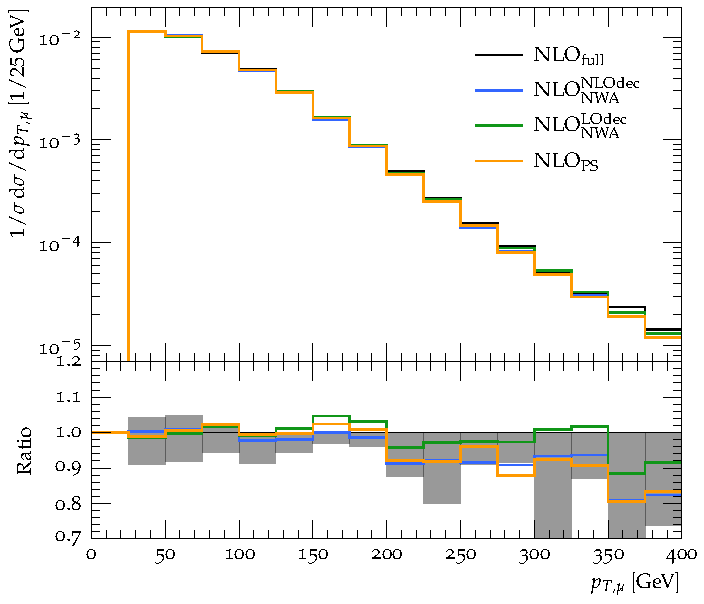
\includegraphics[width=\textwidth]{{plots/scalevarcompare.pTmu}.pdf}
\vspace{\TwoFigBottom em}
\caption{\label{fig:scalevar_ptmu}}
\end{subfigure}
\caption{Normalised differential cross sections for
  (a)~the rapidity of the muon, $\eta_{\mu}$, and
  (b)~the transverse momentum of the muon, $p_{T,\mu}$.
  The ratios of different theoretical descriptions to $\nlofull$
  including its scale uncertainty band are also shown.}
\end{figure}

In Figs.~\ref{fig:scalevar_etamu} and~\ref{fig:scalevar_ptmu}, we show the muon rapidity $\eta_{\mu}$ and the muon transverse momentum $p_{T,\mu}$, respectively.
Our four theoretical predictions for the $(e^+ \nu_e)\,(\mu^- \bar{\nu}_{\mu})\,b\bar{b}$ final state show a rather different behaviour in these two distributions.
While the whole rapidity spectrum in Fig.~\ref{fig:scalevar_etamu} is properly modelled by all predictions,
the transverse momentum spectrum in Fig.~\ref{fig:scalevar_ptmu} is significantly softer in the tail for the $\nlodec$ and $\nlops$ calculations with respect to $\nlofull$.
A possible interpretation is that non-resonant contributions in $\nlofull$ contain $W$-bosons stemming from a
hard collision rather than the top quark decay. Therefore they can carry higher energies which lead to a harder transverse momentum spectrum of the muon.


\subsubsection{Scale dependence at LO and NLO}
\label{subsec:scaledep}

In this section, we will only consider the observables $\mlb$, $\mtwo$, $\mll$ and $\etdr$, as they are promising with respect to
at least one of the requirements of being observables with small systematics and/or high sensitivity to the top quark mass.

For $\nlofull$, we compare LO and NLO predictions on the left-hand side, while in the figures on the right-hand side, we compare the three calculations based on the NWA,
including scale variations.
We observe that the NLO corrections in the $\nlofull$ case lead to significant shape differences compared to $\lofull$,
see Figs.~\ref{fig:mlb_scalevar} to~\ref{fig:ETdR_scalevar}.
While this is to be expected in the tails of the distributions, it is
remarkable that the shape difference also affects the central and in particular the regions with low values of the observables.
Given that the differences between the LO and NLO theory predictions in the full $W^+W^-b\bar{b}$ calculation are still sizeable in the bulk of the distributions, large
differences in the top quark mass extracted from templates based on these predictions can be expected.
The shape differences at low values of $\mlb$ and $\mtwo$ are  less pronounced in the calculations based on the NWA,
as can be seen from Figs.~\ref{fig:mlb_scalevar_nwa}  and~\ref{fig:mt2_scalevar_nwa}.
However, there are also significant shape differences in the bulk of the distribution.
In addition, for the $\mlb$ distribution, Fig.~\ref{fig:mlb_scalevar_nwa}, the peak is lower in the $\nlodec$ and the $\nlops$ case
 compared to the $\lodec$ case, which can be easily understood considering the fact that  more radiation, i.e.~a harder distribution in the tail,
softens the peak region.


\begin{figure}[tbp!]
\centering
\begin{subfigure}{0.495\textwidth}
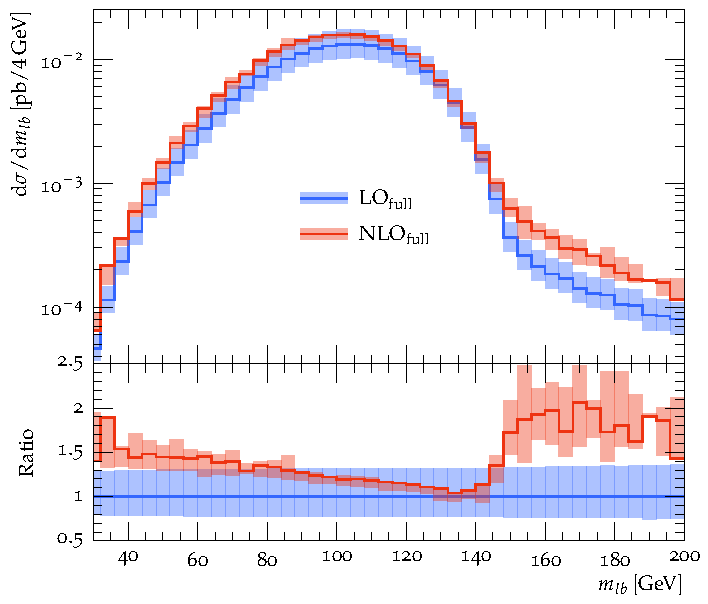
\includegraphics[width=\textwidth]{{plots/scalevar_lo_nlo.wwbb.mlb}.pdf}
\vspace{\TwoFigBottom em}
\caption{\label{fig:mlb_scalevar}}
\end{subfigure}
\hfill
\begin{subfigure}{0.495\textwidth}
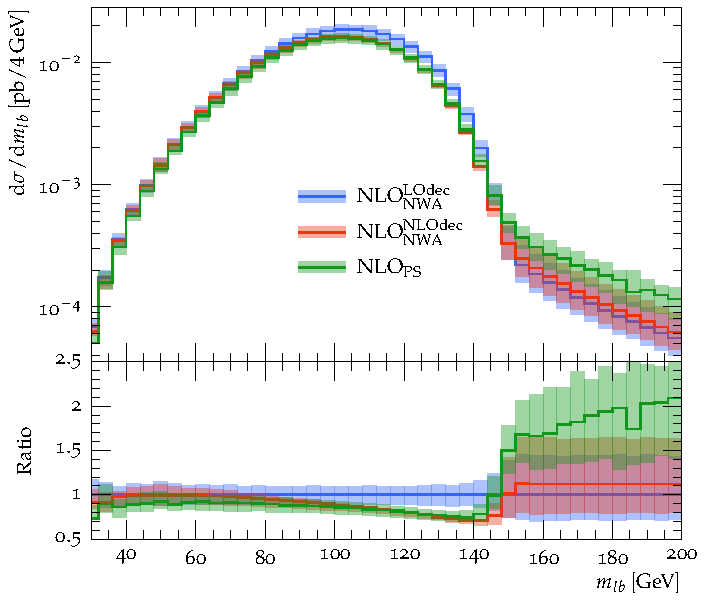
\includegraphics[width=\textwidth]{{plots/scalevar_lo_nlo.nwaps.mlb}.pdf}
\vspace{\TwoFigBottom em}
\caption{\label{fig:mlb_scalevar_nwa}}
\end{subfigure}
\caption{Results including scale variation bands for $m_{lb}$, for (a)~the $\lofull$ and $\nlofull$ calculations, (b)~the calculations based on the NWA.
The ratios with respect to (a) $\lofull$ and (b) $\lodec$ are also shown.\label{fig:mlb_scalevar_all}}
\end{figure}

\begin{figure}[tbp!]
\centering
\begin{subfigure}{0.495\textwidth}
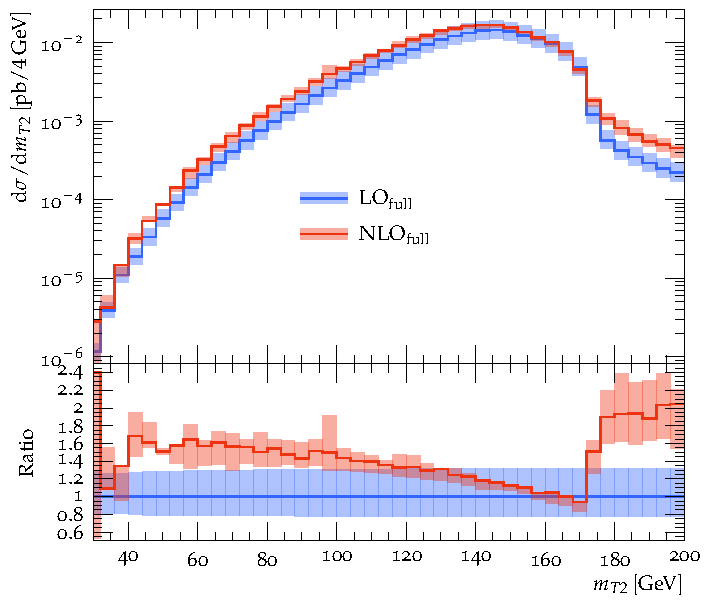
\includegraphics[width=\textwidth]{{plots/scalevar_lo_nlo.wwbb.mt2}.pdf}
\vspace{\TwoFigBottom em}
\caption{}
\label{fig:mt2_scalevar}
\end{subfigure}
\hfill
\begin{subfigure}{0.495\textwidth}
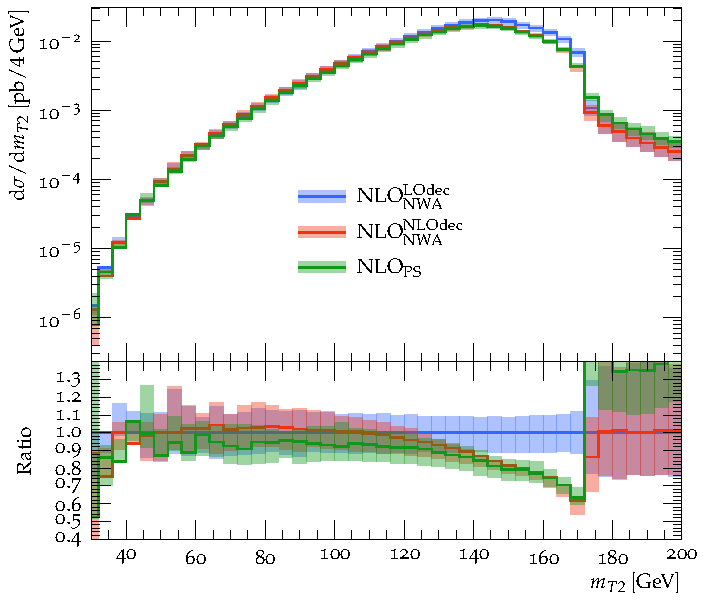
\includegraphics[width=\textwidth]{{plots/scalevar_lo_nlo.nwaps.mt2}.pdf}
\vspace{\TwoFigBottom em}
\caption{}
\label{fig:mt2_scalevar_nwa}
\end{subfigure}
\caption{Results including scale variation bands for $m_{T2}$, for (a)~the $\lofull$ and $\nlofull$ calculations, and (b)~the calculations based on the NWA.
The ratios are defined as in Fig.~\ref{fig:mlb_scalevar_all}.}
\end{figure}



\begin{figure}[tbp!]
\centering
\begin{subfigure}{0.495\textwidth}
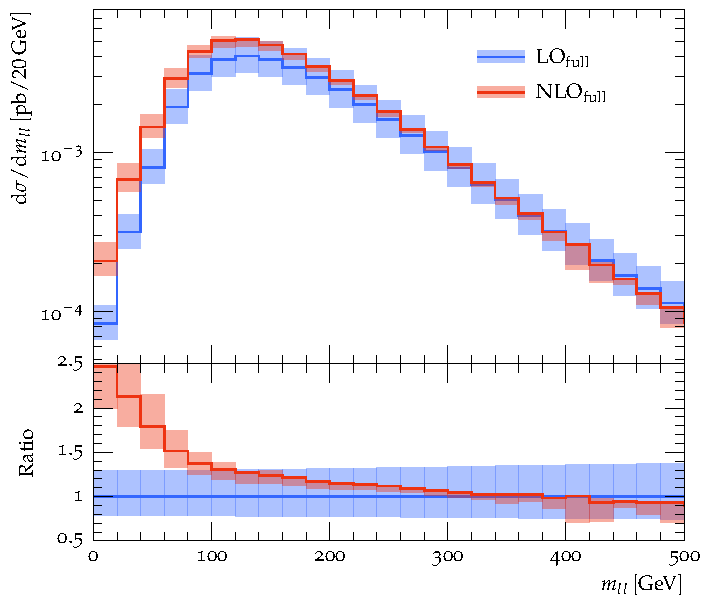
\includegraphics[width=\textwidth]{{plots/scalevar_lo_nlo.wwbb.mll}.pdf}
\vspace{\TwoFigBottom em}
\caption{}
\label{fig:mll_scalevar}
\end{subfigure}
\hfill
\begin{subfigure}{0.495\textwidth}
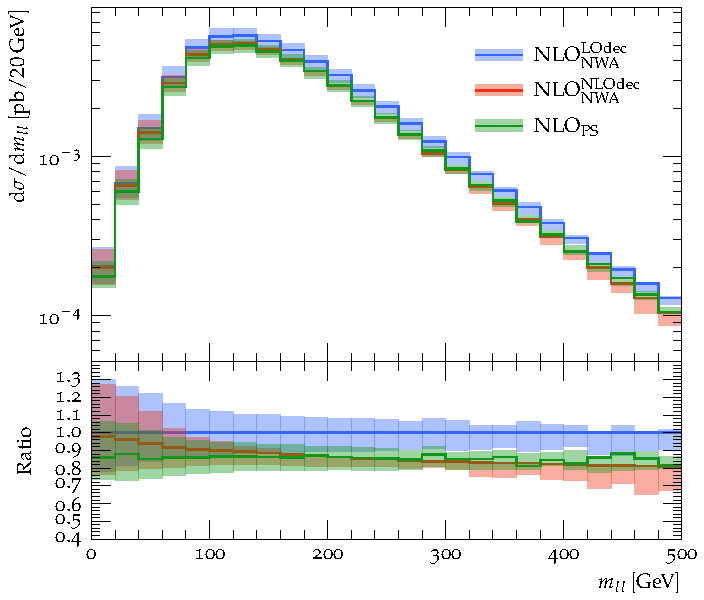
\includegraphics[width=\textwidth]{{plots/scalevar_lo_nlo.nwaps.mll}.pdf}
\vspace{\TwoFigBottom em}
\caption{}
\label{fig:mll_scalevar_nwa}
\end{subfigure}
\caption{Results including scale variation bands for  $m_{ll}$, for (a)~the $\lofull$ and $\nlofull$ calculations, and (b)~the calculations based on the NWA.
The ratios are defined as in Fig.~\ref{fig:mlb_scalevar_all}.}
\end{figure}

\begin{figure}[tbp!]
\centering
\begin{subfigure}{0.495\textwidth}
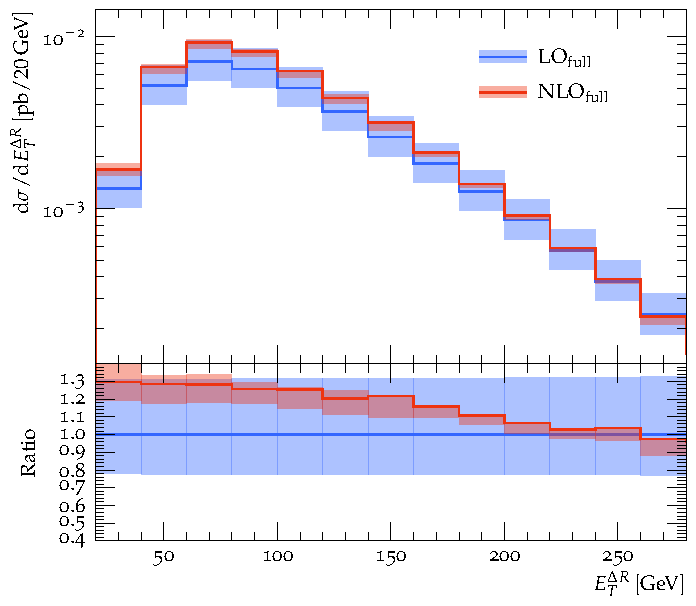
\includegraphics[width=\textwidth]{{plots/scalevar_lo_nlo.wwbb.etdr}.pdf}
\vspace{\TwoFigBottom em}
\caption{}
\label{fig:ETdR_scalevar}
\end{subfigure}
\hfill
\begin{subfigure}{0.495\textwidth}
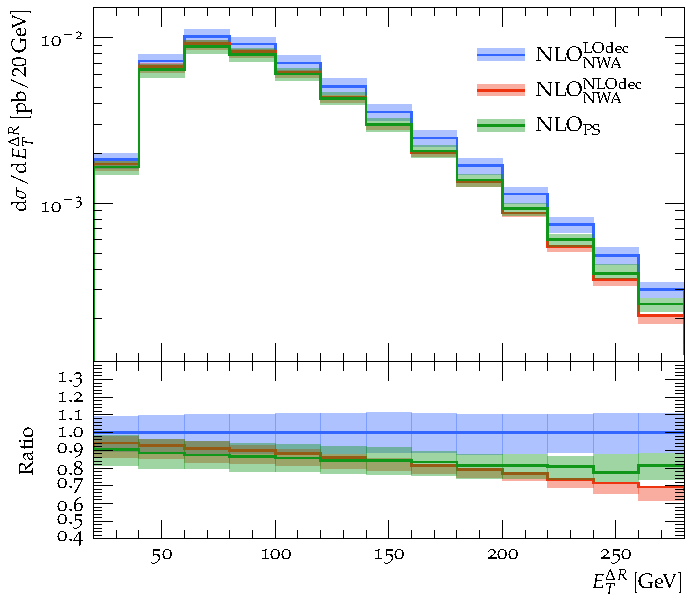
\includegraphics[width=\textwidth]{{plots/scalevar_lo_nlo.nwaps.etdr}.pdf}
\vspace{\TwoFigBottom em}
\caption{}
\label{fig:ETdR_scalevar_nwa}
\end{subfigure}
\caption{Results including scale variation bands for \etdr for (a)~the $\lofull$ and $\nlofull$ calculations, and (b)~the calculations based on the NWA.
The ratios are defined as in Fig.~\ref{fig:mlb_scalevar_all}.}
\end{figure}

For the observable $\mll$, the shape differences introduced by the $\nlofull$ calculation at low $\mll$ values are
particularly pronounced in Fig.~\ref{fig:mll_scalevar}.
The calculations based on the NWA in Fig.~\ref{fig:mll_scalevar_nwa},
$\nlodec$ and $\lodec$, cease to overlap at relatively low $\mll$
values ($\mll\sim160\gev$), while
$\nlops$ mostly lies between $\nlodec$ and $\lodec$ in the region
beyond $\mll>200\gev$.
As shown in Table~\ref{tab:xs}, the total
cross section predicted by $\nlops$ is considerably smaller.
This is due to the fact that after the shower, the $b$-jets are softer and therefore a larger fraction of events does not pass the requirement of
two $b$-jets above $p_{T,\mrm{min}}^\mrm{jet}=25\gev$.
Even though the observable $\mll$ does not involve jets, the jet requirements affect this observable,
since we use the data set produced with the same requirements as for the other observables.
A similar pattern is seen in the observable \etdr (Figs.~\ref{fig:ETdR_scalevar} and~\ref{fig:ETdR_scalevar_nwa}).

The scale variation bands in the $\nlofull$ case and the $\nlodec$ case are rather asymmetric:
the central scale leads to the largest differential cross section compared to up- and downwards variations over a large kinematic range of the corresponding observable.
This effect is particularly pronounced for the $\mll$ and \etdr distributions.


\subsubsection{Distributions for several top quark masses}

\begin{figure}[tbp!]
\centering
\begin{subfigure}{0.495\textwidth}
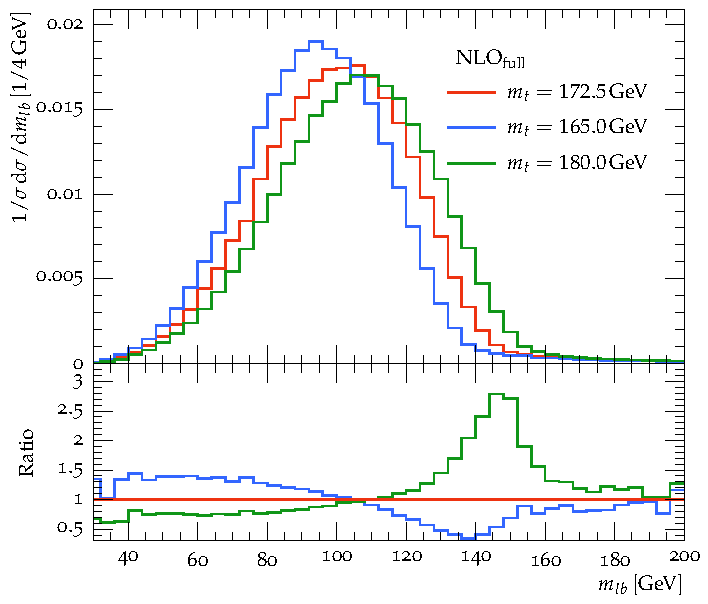
\includegraphics[width=\textwidth]{{plots/massvarcompare.mlb}.pdf}
\vspace{\TwoFigBottom em}
\caption{\label{fig:massvar_fullNLO_mlb}}
\end{subfigure}
\hfill
\begin{subfigure}{0.495\textwidth}
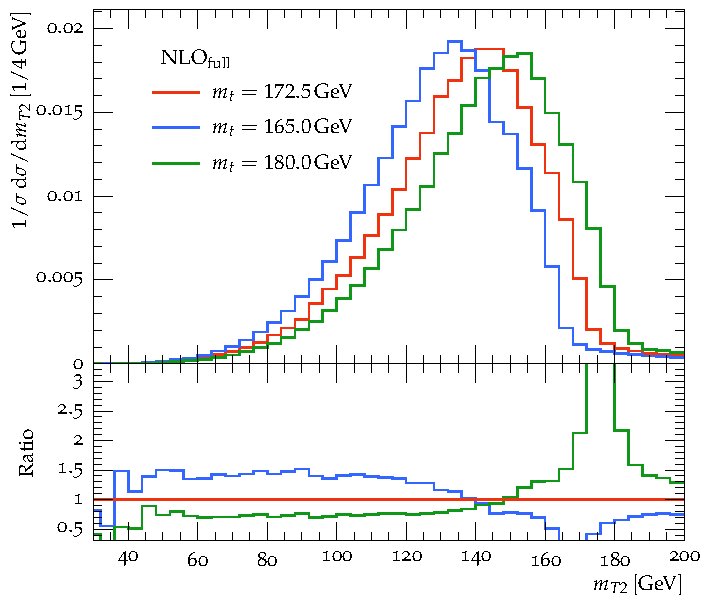
\includegraphics[width=\textwidth]{{plots/massvarcompare.mt2}.pdf}
\vspace{\TwoFigBottom em}
\caption{\label{fig:massvar_fullNLO_mt2}}
\end{subfigure}
\caption{Effect of top quark mass variations on the normalised differential cross sections for $m_{lb}$ and $m_{T2}$.
We also show the ratios to the prediction obtained with $m_t=172.5\gev$.
All results are obtained with the $\nlofull$ description for the $13\tev$ LHC.}
\end{figure}

\begin{figure}[tbp!]
\centering
\begin{subfigure}{0.495\textwidth}
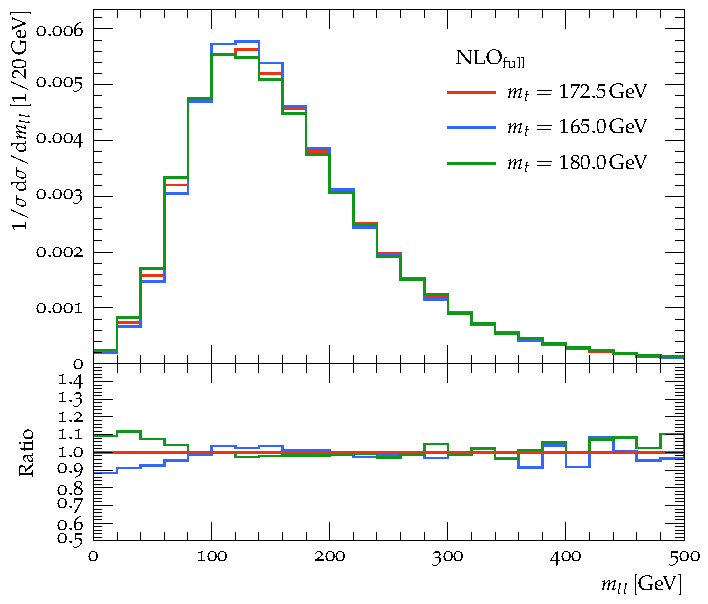
\includegraphics[width=\textwidth]{{plots/massvarcompare.mll}.pdf}
\vspace{\TwoFigBottom em}
\caption{}
\label{fig:massvar_fullNLO_mll}
\end{subfigure}
\hfill
\begin{subfigure}{0.495\textwidth}
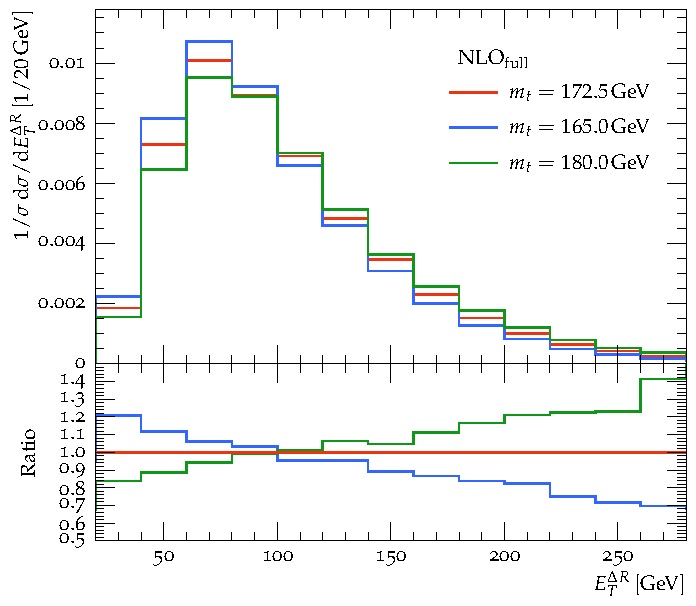
\includegraphics[width=\textwidth]{{plots/massvarcompare.etdr}.pdf}
\vspace{\TwoFigBottom em}
\caption{}
\label{fig:massvar_fullNLO_etdr}
\end{subfigure}
\caption{Effect of top quark mass variation on the normalised differential cross section for $m_{ll}$ and \etdr.
We also show the ratios to the prediction obtained with $m_t=172.5\gev$.
The results are obtained with the $\nlofull$ description for the $13\tev$ LHC.}
\end{figure}

In this section, we investigate the sensitivity of the four observables $\mlb$, $\mtwo$, $\mll$ and $\etdr$ to variations of the top quark mass.
We exploit distributions based on the $\nlofull$ calculation using the three values,
$m_t=165$, $172.5$, $180\gev$, for the top quark mass.

We observe a strong sensitivity of the $\mlb$ and $\mtwo$ distributions to the top quark mass
with ratios up to about three in the given range.
A lower top quark mass naturally leads to a softer spectrum while a higher top quark mass leads to a harder spectrum in these two observables.
The sensitivity of $\mll$ is shown in Fig.~\ref{fig:massvar_fullNLO_mll} and turns out to be very small.
Unfortunately, being a purely leptonic observable,
the low sensitivity counterbalances its expected~\cite{Frixione:2014ala} better experimental systematics.
Compared to the $\mll$ distribution, the \etdr distribution in Fig.~\ref{fig:massvar_fullNLO_etdr} shows a somewhat larger sensitivity to $m_t$, albeit much smaller than what is observed for $\mlb$ and $\mtwo$.
